\documentclass{article}

\usepackage[%
    left=0.5in,%
    right=0.5in,%
    top=0.5in,%
    bottom=0.5in,%
]{geometry}%
\usepackage{minitoc}
\usepackage{multicol}
\usepackage{graphicx}
\usepackage{fixltx2e}
\usepackage{listings}
\usepackage{color}
\usepackage{amsmath}
\usepackage{hyperref}
    \hypersetup{ colorlinks = true, linkcolor = blue }
\usepackage{blindtext}
\definecolor{lightgray}{gray}{0.9}
\graphicspath{ {./} }

\newcommand{\inlinecode}[2]{\colorbox{lightgray}{\lstinline
[language=#1]$#2$}}
\newcommand{\worddef}[1]{\hyperref[sec:reference]{\textit{#1}}}

\begin{document}

\tableofcontents

\newpage

\section{Public key cryptography}
\begin{itemize}
  \item Two keys, a public key and a private key 
  \item Public-key (asymmetric) cryptography hinges upon the premise that: \textbf{It is computationally infeasible to calculate a private from a public key}
  \item Public-key cryptography gains us a few important abilities:
  \begin{itemize}
    \item We can exchange a private symmetric key “in the open” 
    \item We can verify the sender of a message 
    \item Non-repudiation – you can’t deny you did something
  \end{itemize}
\end{itemize}
\begin{center}
  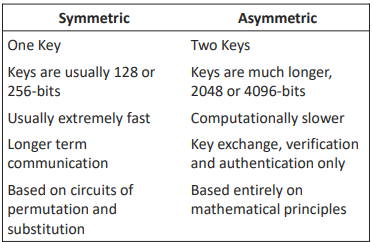
\includegraphics[scale=0.5]{sym_vs_asym_keys.png}
\end{center}

\section{Big numbers}
\begin{itemize}
  \item Modular \textbf{arithmetic} and \textbf{integer factorisation} drive public-key cryptography
  \item As computer power increases, we can increase the size of these numbers to preserve the integrity of our algorithms
\end{itemize}

\section{Modular Arithmetic}
\begin{flushleft}
A system of arithmetic based around \textbf{cycles of numbers}. Numbers modulo n are a \worddef{finite field}. Can think of it as a circle, because the set of numbers is limited and goes in a loop
\end{flushleft}

\subsection{The Congruence Relation}

\begin{flushleft}
For a positive integer $n$, two numbers $a$ and $b$ are said to be \textit{congruent modulo} $n$, if their difference $a − b$ is an integer \textbf{multiple} of $n$ (that is, if there is an integer k such that $a − b = k*n$). This congruence relation is typically considered when a and b are integers, and is denoted
\end{flushleft} 
\begin{gather}
  a\equiv b \kern-0.3cm \pmod{n} \\
  a \kern-0.3cm \pmod{n} = b \kern-0.3cm \pmod{n}
\end{gather}

\begin{flushleft}
When you apply modulo makes no difference
\end{flushleft}
\begin{gather}
  ((a \kern-0.3cm \mod{n}) + (b \kern-0.3cm \mod{n})) \kern-0.3cm \mod{n} = (a + b) \kern-0.3cm \mod{n} \\
   ((a \kern-0.3cm \mod{n}) * (b \kern-0.3cm \mod{n})) \kern-0.3cm \mod{n} = (a * b) \kern-0.3cm \mod{n}
\end{gather}

\pagebreak

\subsection{Logarithms}
\begin{flushleft}
A logarithm is the inverse function to exponentiation
\begin{gather}
   a^{b} = c \\
   b = log_a c
\end{gather}
\end{flushleft}

\begin{flushleft}
When operating $\mod n$, we call the operation a discrete logarithm. Discrete logs are much harder to compute. The number that is raised to a certain power, is called the \textbf{generator g}
\end{flushleft}

\begin{center}
  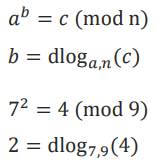
\includegraphics[scale=0.5]{dlog.png}
\end{center}

\section{Diffie-Hellman}
\begin{itemize}
  \item Two parties can jointly agree a \textit{shared secret} over an insecure channel 
  \item Mathematically, what we are doing is both calculating the same value, mod a prime p
  \item Look at \href{https://moodle.nottingham.ac.uk/pluginfile.php/5121129/mod_resource/content/0/L5%20-%20Cryptography%20III%202pp.pdf}{notes}:
\end{itemize}

\subsection{Why is DH KEX Secure?}
\begin{itemize}
  \item The secret shared key is gab 
  \item Yet, only g, p, g a and g b have been transmitted and are public 
  \item The only way to calculate $g^{ab}$ is either $(g^a)^b$ or $(g^b)^a$ 
  \item The only way to find a or b is solve:
\end{itemize}

\begin{center}
  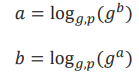
\includegraphics[scale=0.5]{solver.png}
\end{center}


\subsection{Vulnerabilities}
\begin{flushleft}
Man-in-the-middle: A third party could intercept the initial communication from Alice, then create two separate key exchanges with both Alice and Bob. \textbf{An asymmetric protocol is required to prevent this}
\end{flushleft}

\subsection{Perfect Forward Secrecy}
\begin{itemize}
  \item There’s always a chance a DHKEX key might be broken 
  \item If we establish a symmetric key, how long should we use it for? 
  \item Perfect forward secrecy means we \textbf{generate new keys for each session}, rather than persistent keys
\end{itemize}

\subsection{Ephemeral Mode}
\begin{itemize}
  \item In protocols like TLS, running Diffie-Hellman in ephemeral mode forces a new key exchange every time 
  \item The recommended settings for TLS are now 2048-bit DH keys, in ephemeral mode
\end{itemize}

\section{Elliptic Curve Cryptography}
\begin{flushleft}
Elliptic curves, of the form $y^2 = x ^3 + ax + b$ can be used in place of mod arithmetic in DHKEX
Elliptic curves are much stronger than traditional public-key schemes for the \textbf{same key length}
\end{flushleft}

\pagebreak

\section*{Reference section} \label{sec:reference}
\begin{description}
	\item[finite field] \hfill \\ A finite field is a set of numbers in which we can add, subtract, multiply and divide, and stay within that set
\end{description}
\end{document}
